\documentclass[12pt]{article}
\usepackage{amsfonts}
\usepackage{mathtools}
\usepackage{fontspec}
\usepackage{physics}
% \usepackage[left=1.06cm,top=0.9cm,right=1.06cm,bottom=0.49cm]{geometry}
% \setmainfont{GFS Didot}
\setmainfont{EB Garamond}


% Set page size and margins
% Replace `letterpaper' with `a4paper' for UK/EU standard size
\usepackage[a4paper,top=2cm,bottom=1.5cm,left=1cm,right=1cm]{geometry}
\usepackage{fancyhdr}
\pagestyle{fancy}
\setlength{\parindent}{0pt}


% Useful packages
\usepackage{graphicx}
\graphicspath{{./media/}}
\usepackage{subcaption}
\usepackage{float}
\usepackage[colorlinks=true, allcolors=blue]{hyperref}
\usepackage{siunitx}
\usepackage{sectsty}
\sectionfont{\fontsize{12}{15}\selectfont}
\renewcommand{\labelenumi}{\alph{enumi})}

\title{\vspace{-2cm} Stochastic Control \\ 
        \large Homework Project 2 \\
        Reinforcement Learning with Policy Gradient}
\author{Ioannis Dimoulios \\ 
        \small Mat. Num. 470364}
\date{Winter Semester 2024}

\lhead{Stochastic Control}
\chead{Homework Project 2}
\rhead{Ioannis Dimoulios}
\begin{document}
\maketitle

\section*{Problem 1}
a) Simple algebraic manipulation yields 
\begin{equation*}
    \xi(t_{k+1}) = \underbrace{\xi(t_{k}) + 0.2\delta t \begin{bmatrix}
        -\sin(\frac{t_k}{50}) \\ +\cos(\frac{t_k}{50})
    \end{bmatrix}}_{f_1(\xi(t_k), t_k)} + \begin{bmatrix}
        w_1(t_k) \\ w_2(t_k)
    \end{bmatrix}
\end{equation*}
Now taking into account that \(w \sim \text{Laplace}(0, \sigma)\), we get that 
\begin{equation*}
    \rho_1(\xi(t_{k+1}) | \xi(t_k), t_k) \sim \text{Laplace}(f_1(\xi(t_k), t_k), \sigma), 
\end{equation*}
which holds per coordinate. 

b) In similar fashion 
\begin{gather*}
    \zeta(t_k) = \xi(t_k ) + \begin{bmatrix}
        v_1(t_k) \\ v_2(t_k)
    \end{bmatrix} \\
    \rho(\zeta(t_k) | \xi(t_k)) \sim \mathcal{U}(\xi(t_k) - \varepsilon, \xi(t_k) + \varepsilon), 
\end{gather*}
which again holds per coordinate. 

\section*{Problem 2} 
a) Monte Carlo integration conveys the simple idea, that if we cannot analytically calculate the expected value of a random variable, we can just draw various realizations of the random variable. Then, their average will converge to the expected value as the number of samples grows. 

Importance sampling on the other hand says that if we do cannot draw samples from this particular distribution \(\rho(\cdot)\), but we have a good enough approximation distribution \(\mu(\cdot)\) (importance density), then we may as well draw samples from the approximation. In this case, as long as we take the weighted mean of the samples the estimate will still be a good approximation of the expected value. Each weight corresponds to the value 
\begin{equation*}
    w^{(i)} = \dfrac{1}{N }\dfrac{\rho(\xi^{(i)})}{\mu(\xi^{(i)})}, 
\end{equation*}
where \(N \) is the number of samples and \(\xi^{(i)}\) the \(i\)-th sample. \\

b) State estimation essentially requires that we find the unknown state which evolves over time when we know that each moment it follows a particular distribution, and we have prior information of the output of the system, i.e. noisy measurements of a function of the state. To do this, we use the particle filter which provides a systematic way to sample a good enough approximation of the distribution of the state, which evolve over time employing the system dynamics, and calculate reliable weights to get a weighted average of the samples which in theory should be a good approxiamation of the current state. 

// TODO: explain in detail each step of the particle filter. \\

c) To begin with, \(x_k \) corresponds to \(\xi(t_k) \). Note that there is no input, i.e. the system is autonomous. 

Then, \(z_k \) corresponds to \(\zeta(t_k )\). \\

d) The obvious way to choose \(q(\cdot )\) is 
\begin{equation*}
    q(x_k^{(i)}|x_{k-1}^{(i)}, u_{k-1}) = \rho(x_k^{(i)}|x_{k-1}^{(i)}, u_{k-1}). 
\end{equation*}
This simplifies the calculation of the next batch of weights, as 
\begin{equation*}
    w_k^{(i)} = \rho(z_k|x_k^{(i)})w_{k-1}^{(i)}. 
\end{equation*}

An alternative would be to simply let \(q(\cdot )\) be a Gaussian distribution. In that sense, 
\begin{equation*}
    q(x_k^{(i)}|x_{k-1}^{(i)}, u_{k-1}) \sim \mathcal{N}(x_k^{(i)}; f(x_{k-1}^{(i)}, u_{k-1}), \Sigma_k), 
\end{equation*}
where \(f(\cdot )\) is the system dynamics function excluding the non-predictable factor and \(\Sigma_k \) is the to be determined covariance matrix. 

\section*{Problem 3}
a) Pretty much done already in Problem 1. \\

b) We chose the first option outlined in 2d. \\

c) See source code, namely file \texttt{src/particle\_filter.jl} \\

\begin{figure}[H]
    \centering
    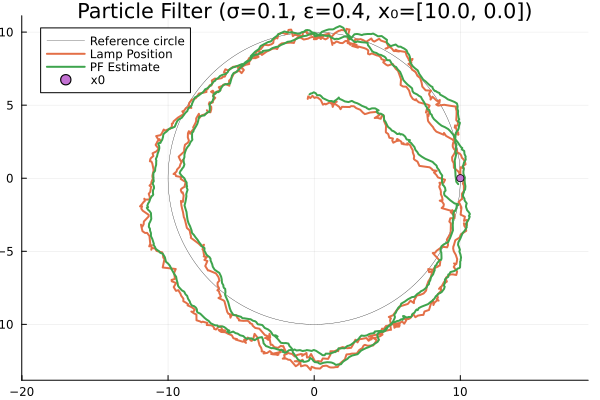
\includegraphics[width=0.7\textwidth]{3a.png}
\end{figure} 
\begin{figure}[H]
    \centering
    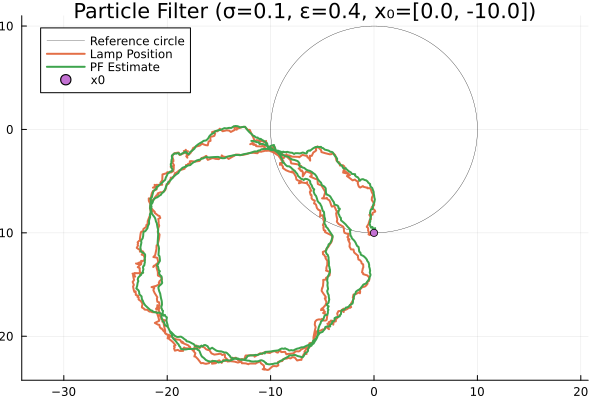
\includegraphics[width=0.7\textwidth]{3b.png}
\end{figure}  
\begin{figure}[H]
    \centering
    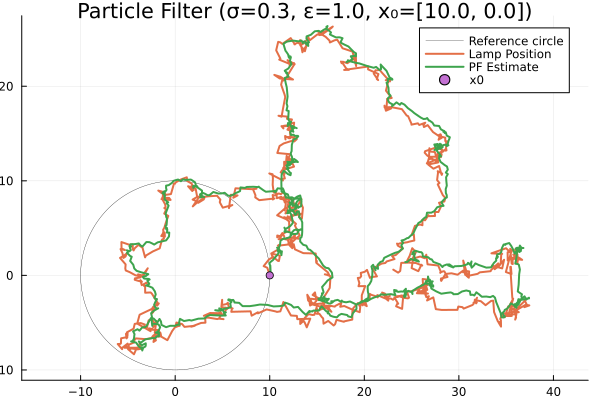
\includegraphics[width=0.7\textwidth]{3c.png}
\end{figure} 
\begin{figure}[H]
    \centering
    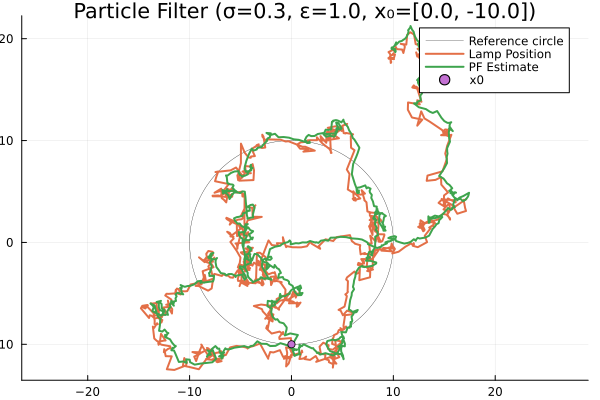
\includegraphics[width=0.7\textwidth]{3d.png}
\end{figure} 

\section*{Problem 4}
a) In similiar fashion to the discretization in Problem 1, 
\begin{gather*}
    \dv{\theta}{t} = u \\ \implies \theta_{k+1} - \theta_k = u_k\delta t \\
    \implies \theta_{k+1} = \theta_k + u_k\delta t. 
\end{gather*}

b) We basically want \(u \propto \hat{\xi}_k - \theta_k \) where \(\hat{\xi}_k\) is the calculated estimate for \(\xi_k \) provided by the particle filter and simultaneously \(\|u\|_2 \leq 1\). Hence, simply 
\begin{equation*}
    u = \dfrac{\hat{\xi}_k - \theta_k}{\max(\|\hat{\xi}_k - \theta_k\|, 1)}.
\end{equation*}

c) See source code, namely file 
\texttt{src/source\_seeking.jl}. \\

d) It works quite well. Maybe the maximum magnitude of the velocity is a little too big and the robot sometimes unnecessarily jiggles trying to mimic the minor displacements of the lamp due to the disturbances in its dynamics. \\

We have lowered the maximum speed (norm of velocity) of the robot, so that its graph is a little bit smoother. \\
See the included \texttt{.gif} files for the moving plots. 

\end{document}

